\documentclass[11pt]{article}

% the percent sign gives comments in Latex
% top line indicates this is for Physical Review, standard journal format,
% suitable for electronic submission of articles

% the line above is necessary to start any latex document.
% this is one variation that should work for most things.
% if you want double spaceing, use the following:
%
%\documentclass[prd,preprint,letterpaper]{revtex4}
%
% the "preprint" designation will make a wider line
% spacing, good for markup.
\usepackage{graphicx}  % this is the up-to-date package for all figures
\usepackage{float}	% allows use of 'H' command

% these are some custom control of the page size and margins
% \topmargin= 0.2in  % these 1st two may be needed for some computers
%\textheight=8.75in
\textwidth=6.5in
\oddsidemargin=0cm
\evensidemargin=0cm

% this is where the actual document itself (rather than control statements) begins:

\begin{document}

% use a style that gives automatic headings
\pagestyle{myheadings}

% the \title{} command generates a title.

% the \\ below is used to FORCE a line break in the middle of the sentence--
% otherwise latex computes it for you

\title{Lab 6:\\
Carbon Isotope Decay}


\author{Corey Mutnik \\
{\it Computational Physics 305, University of Hawaii at Manoa} }


\date{March 3, 2015}




\maketitle    % this line is necessary to tell latex you are done with all
	      % of the stuff associated with the title, and now it can go
              % ahead and generate the title portion


	      % \section is used to start a new one with a heading
\abstract{
All living matter contains isotopes of Carbon.  In knowing Carbon to have a specific decay rate, one is able to determine 
the age of biomass samples.  This technique is know as Carbon-dating.  The decay of such isotopes is seemingly random 
but occurs with an overall average.  Such an average rate is fitted to a known distribution in order to use it in making 
various other calculations and predictions.
}

\section{Introduction}

Patterns often arise from seemingly random collections of data.  An example of this, used in lab 6a, is the 
counting of meteor sightings during a portion of a meteor shower.  Such a collection of data seems random since 
sightings are not guaranteed to occur at evenly spaced time intervals.  From these recordings a time series was 
generated.  Such data becomes more useful when it is re-binned (grouped) into quantized time packets.  Although 
the raw data may make predicting when any given meteor will be recorded nearly impossible, it is useful once 
patterns across segments of time are analyzed.  From such analysis, distribution patterns emerge.



Although a variety of distributions exist, this lab focused on the Poisson distribution.  This particular 
distribution was chosen due to how well it represented our collected data.  This was verified by fitting a 
Poisson distribution curve to our data points (equation 2).  The Poisson distribution equation was normalized in order to 
always generate a net probability of 1 (equation 1).



The techniques learned in the first portion of this lab are utilized in the later portion, when analyzing 
the decay of unstable carbon isotopes.  Poisson distribution fits using the Von Neumann method will be used to determine the 
accuracy of estimated ages for specific biomaterial.  This is seen through the relative abundance of the remaining $C_{14}$ 
isotope within a given sample.


% one or more lines of space between paragraphs determines them
\section{Code}

Various programs and plot files can be seen online at: \\
http://www2.hawaii.edu/$\sim$cmutnik/lab6.html


\section{Computational problem}

In this weeks lab we had to model the decay of unstable carbon isotopes.  The practicality of doing this was shown when 
estimating the age of objects based off the amount of remaining C14 within the object.


The total number of trial minutes recorded in the data set, N, is know.  This allows us to use the normalized 
Poisson:\\
\begin{equation}
\label{NormalizedP}
P(k~:~ \mu,~N) ~=~ N~ \mu^k \frac{e^{-\mu}}{k!}
\end{equation}
Where P is probability, k is an integer, and $\mu$ is the mean number of events in a time interval.


The Poisson function used in fitting the data:
\begin{equation}
\label{fit}
f(x) = N\frac{e^{-\mu}\mu^{x}}{x!}
\end{equation}
Where N is the starting point used as an estimator for the number of trials.


\begin{equation}
\label{decay}
N(t) = N{12} + N{11}e^{-t/T{11}} + N{10}e^{-t/T{10}}
\end{equation}
Where N represents the number of atoms for each isotope of Carbon.  $T_{11}$ and $T_{10}$ are the characteristic 1/e decay 
times for each isotope, respectively.

\section{Graphs}

\begin{figure}[H]
  \begin{center}
\centerline{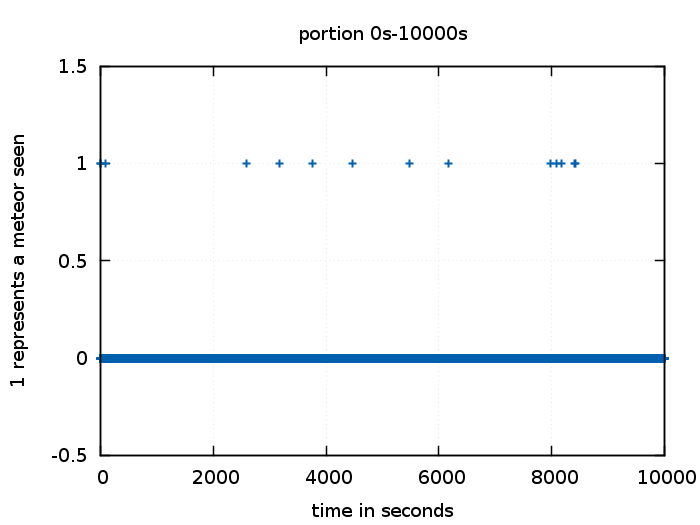
\includegraphics[width=3.75in]{portion0_10000.png}}
\caption{\it \small{Portion of raw meteor sighting data \label{fig1}}}
  \end{center}
\end{figure}

\begin{figure}[H]
  \begin{center}
\centerline{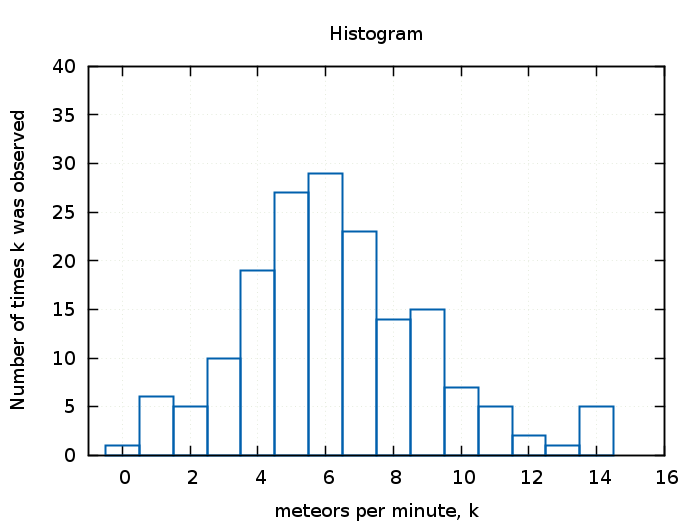
\includegraphics[width=3.75in]{meteorhistogram.png}}
\caption{\it \small{Histogram showing meteors seen organized by time bin \label{fig2}}}
  \end{center}
\end{figure}

\begin{figure}[H]
  \begin{center}
\centerline{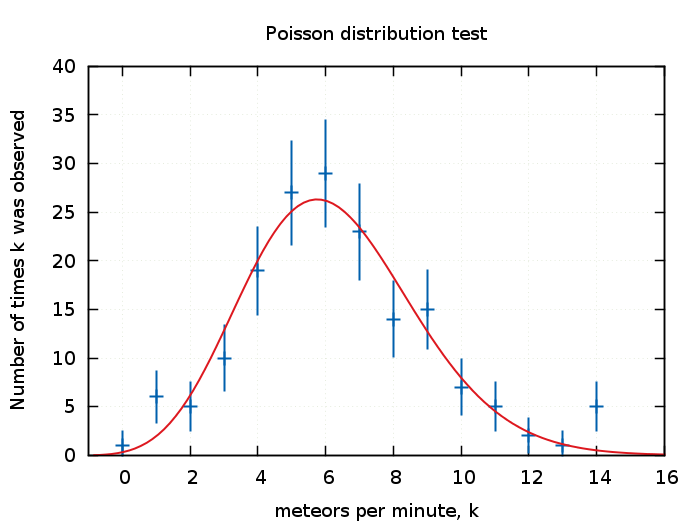
\includegraphics[width=3.75in]{histwitherr.png}}
\caption{\it \small{Portion of raw meteor sighting data \label{fig3}}}
  \end{center}
\end{figure}


\begin{figure}[H]
  \begin{center}
\centerline{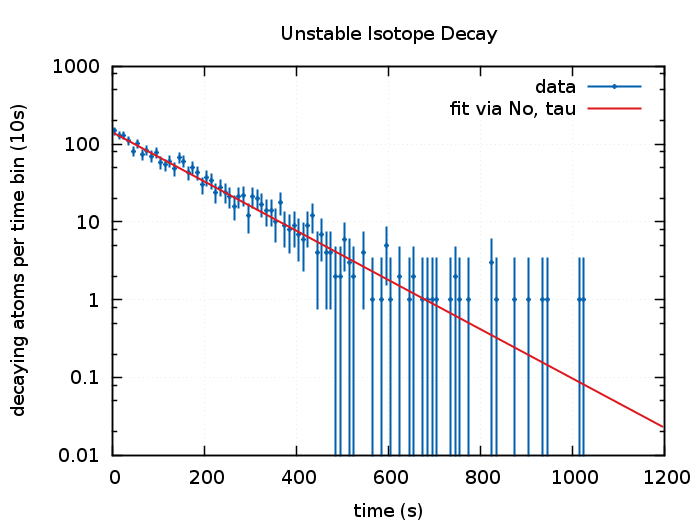
\includegraphics[width=3.75in]{decayfit.png}}
\caption{\it \small{Fitted unstable isotope decay, with bin size of 10 seconds \label{fig4}}}
  \end{center}
\end{figure}

\begin{figure}[H]
  \begin{center}
\centerline{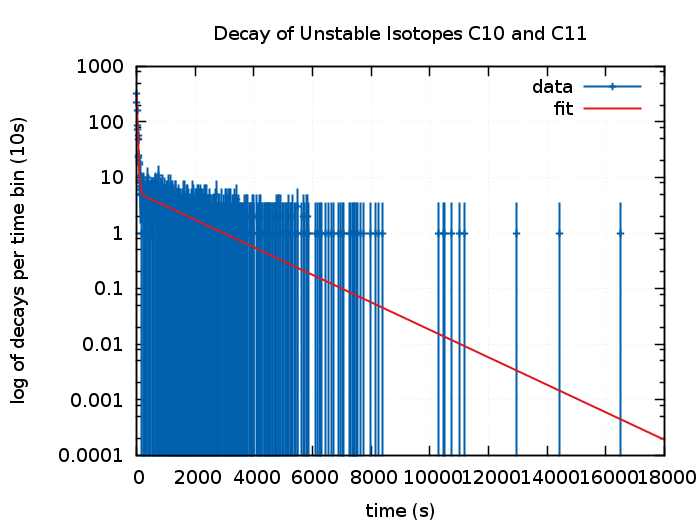
\includegraphics[width=3.75in]{unstabledecaynozoom_1000.png}}
\caption{\it \small{Sum of all the $C_{10}$, $C_{11}$, and $C_{12}$ particles as they decay at different rates; each with an inital sample size of 1000, and time bins of 10 seconds \label{fig5}}}
  \end{center}
\end{figure}

\begin{figure}[H]
  \begin{center}
\centerline{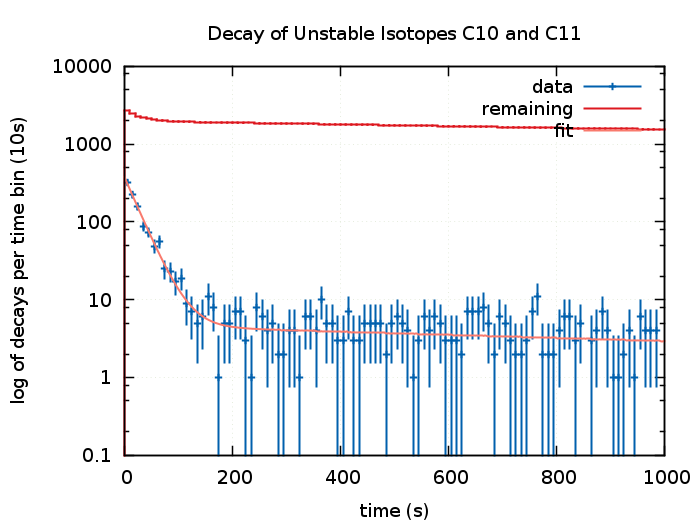
\includegraphics[width=3.75in]{unstabledecayn_1000_withr.png}}
\caption{\it \small{The graph above displays a portion of figure 5, to more easily show the particle decay.  It also plots the remaining number of total Carbon particles as a function of time. \label{fig6}}}
  \end{center}
\end{figure}

\begin{figure}[H]
  \begin{center}
\centerline{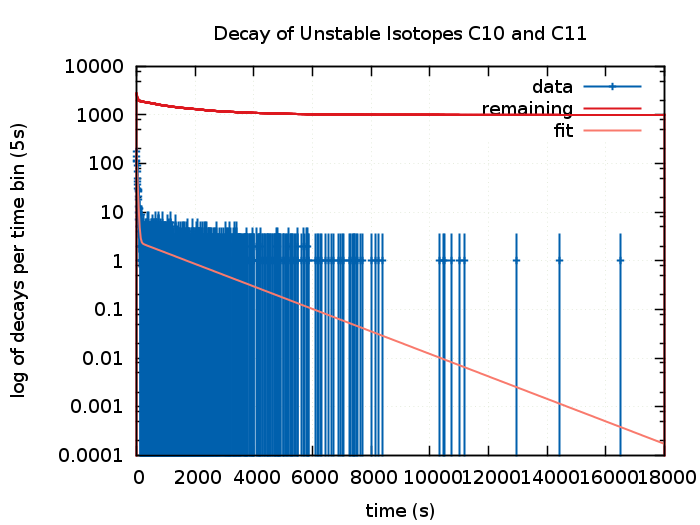
\includegraphics[width=3.75in]{unstabledecaybin5s.png}}
\caption{\it \small{Sum of all the $C_{10}$, $C_{11}$, and $C_{12}$ particles as they decay at different rates; each with an inital sample size of 1000, and time bins of 5 seconds \label{fig7}}}
  \end{center}
\end{figure}

\begin{figure}[H]
  \begin{center}
\centerline{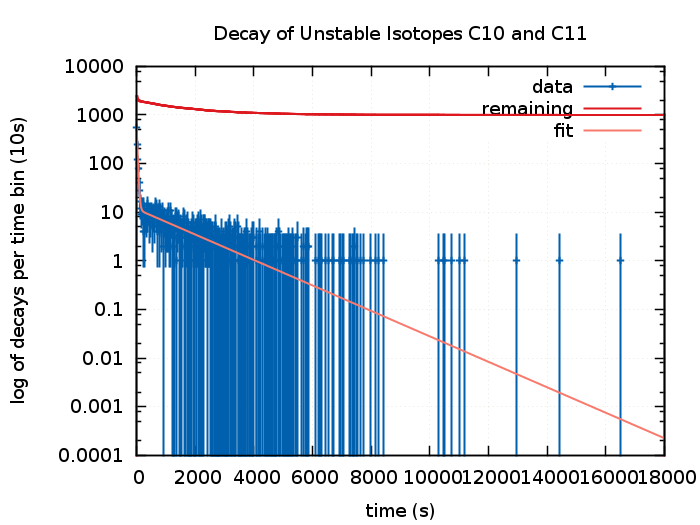
\includegraphics[width=3.75in]{unstabledecaybin20s.png}}
\caption{\it \small{Sum of all the $C_{10}$, $C_{11}$, and $C_{12}$ particles as they decay at different rates; each with an inital sample size of 1000, and time bins of 20 seconds \label{fig8}}}
  \end{center}
\end{figure}

\begin{figure}[H]
  \begin{center}
\centerline{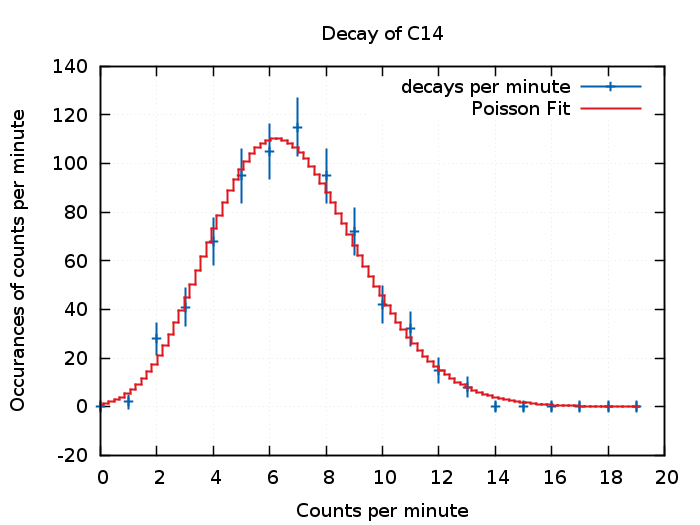
\includegraphics[width=3.75in]{sample1_10000trials.png}}
\caption{\it \small{Sample 1 data with fit, using 10,000 trials \label{fig9}}}
  \end{center}
\end{figure}

\begin{figure}[H]
  \begin{center}
\centerline{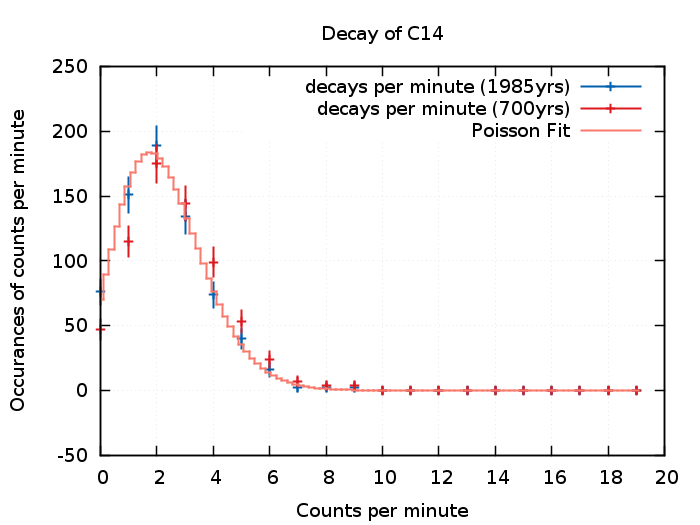
\includegraphics[width=3.75in]{sample2_10000trials.png}}
\caption{\it \small{Sample 2 data with fit, using 10,000 trials \label{fig10}}}
  \end{center}
\end{figure}

\begin{figure}[H]
  \begin{center}
\centerline{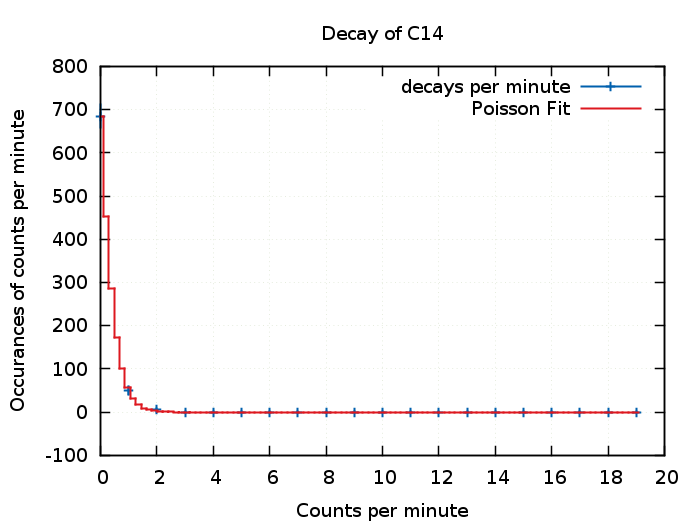
\includegraphics[width=3.75in]{sample3_10000trials.png}}
\caption{\it \small{Sample 3 data with fit, using 10,000 trials \label{fig11}}}
  \end{center}
\end{figure}

\begin{table}[H]
  \begin{center}
\begin{tabular}{|l|c|c|c|}
\hline
                       & \textbf{m} & \textbf{error (+/-)} & \textbf{percent error} \\ \hline
Sample 1               & 6.74887    & 0.0915               & 0.01356                \\ \hline
Sample 2 (700 years)   & 2.68464    & 0.02718              & 0.01012                \\ \hline
Sample 2 (1,985 years) & 2.26839    & 0.02854              & 0.01258                \\ \hline
Sample 3               & 0.0749251  & 0.002581             & 0.03445                \\ \hline
\end{tabular}
\caption{\it \small{This displays the mean decay rates per minute, m, in counts per minute, standar and percent error. \label{table1}}}
  \end{center}
\end{table}

\section{Analysis}

Figure 1 shows a portion of the time spent recoring meteor sightings.  A value of 1, on the vertical axis, is used to indicate 
the time at which each sighting occured.  This data was re-binned for more useful analysis.  Figures 2 and 3 are different 
methods of displaying the same re-binned meteor sighting data, using a histogram.  Figure 2 represents the meteors seen as a 
histogram, showing the number of times a particular amount of meteors was observed.  Figure 3 shows represents this data, 
along with its error, and a Poisson distribution fitted to it.



The program found at:
\begin{center}
http://www2.hawaii.edu/$\sim$cmutnik/isotope2.html
\end{center}
was written using equation 3.  
Figure 5 displays the decay of the Carbon sample.  It uses equation 3 to sum the remaining number of overall Carbon 
partcles, taking into account various decay times.  To generate this plot we assumed $C_{12}$ to be stable and not decay,
$C_{11}$ to have a half-life of 1221 seconds, and $C_{10}$ to have a half-life of 19.29 seconds.  Taking into account that a 
particles decay time is half-life/log(2).  In figure 5 each time bin has a value of 10 seconds.  Since the decay occurs 
so rapidly figure 6 has also been included.  Figure 6 is a zoomed-in portion of figure 5 and displays the total number of 
remaining Carbon particles.  Figure 7 represents the same data as figure 4 but using time bins of 5 seconds each, rather 
than 10 seconds.  Figure 8 represents the same data as figures 4 and 6 but using time bins of 20 seconds each.  The 5 second 
time bin process drastically underestimated the number of inital atoms, while the 20 second time bin process overestimated.  
From this it is easy to conclude that time bins of 10 seconds are optimal, when modeling this process. 



Finally, we simulated a Poisson process in order to calculate the age of certain objects/materials.  Calculating the age 
of each sample is done by measuring the amount of $C_{14}$ reamining in the sample.  We can do this by measuring the activity 
of a sample.  Activity is the number of detected decays of a sample.  This counts are grouped into one minute time intervals.  
This exploits the fact that all biomass contain a certain amount of the $C_{14}$ isotope and $C_{14}$ has a precise activity 
of 15.0 decays per minute per gram.  This required the implementation of the Von Neumann method, which allowed for the 
transfromation of uniform random numbers.
The program used here can be found at:
\begin{center}
http://www2.hawaii.edu/$\sim$cmutnik/C14.html
\end{center}
Figure 9 represents the data from the first sample, a skeletal fragment of Encino Man, which contained 6 grams of 
Carbon and was estimated to be 21,600 years old.  Sample 2, linen of the Shroud of Turin, was estimated to either be 
700 or 1,985 years old.  Both cases were tested and plotted in figure 10.  The discrepancy between the overlaying sets of 
data tells us that if we to take measurments over a longer period of time one ages' data set would better depict our fit.  
Data represented in table 1 shows that, for sample 2, -700 years is a more accurate representation of the age than 1985 years 
old.  It is this age that can be concluded as the more correct estimation.  Sample 3, a sample of hair from an unknown mummy 
contains 10 milligrams (0.01g) of Carbon and is estimated to be 4,700 years old.  Each of these samples was run using 10,000 
trials.  The overlapping of our data with the fitted curve indicates that the estimated ages are accurate.


\section{Conclusion}

The ability to represent data in mulitple fashions is not something that should be over looked.  Raw, collected, data can be 
useful.  But even more so, distributions that arise from properly averaging such data allow accurate predictions to be made.  
By using computational techniques we are able to properly fit data to a variety of distributions.  Such tools are essential 
in deepening our understanding and representation of the physical world.  Modeling known behavior accurately allows the 
predictions of others to be accurate, even if not directly observable.



% the following \setlength is to force the bibliography to have no
% paragraph indentations.Can use vairous units--cm are used here.
\setlength{\parindent}{0cm}

\begin{thebibliography}{99}  % the trailing 99 controls some obscure format--just use

\bibitem{Landau} R. H. Landau and M. J. Paez, "Computational Physics, Problem Solving with Computers,"
(Wiley: New York) 1997.
\\
\bibitem{Gorham} P. Gorham, (2014).
\\
\bibitem{Steve} S. Covin, (2015).
\\
\bibitem{distribution} "Comparison of Distribution Functions." \textit{HyperPhysics}. N.p., n.d. Web. 28 Feb. 2015.


\end{thebibliography}

\end{document}

